\chapter{van Emde Boas Trees}

In Chapter~20, Fibonacci heaps demonstrated how amortized accounting drives insertion and decrease-key down to $O(1)$ time, yet extracting the minimum remained bounded by $\Omega(\log n)$ comparisons. Every comparison-based data structure for maintaining an ordered set---balanced binary search trees, red-black trees, B-trees, or heaps---must charge $\Omega(\log n)$ to locate or extract a key, bounded by the information-theoretic floor on pairwise comparisons.

What happens if keys are not abstract objects, but integers drawn from a known, bounded range $\{0, 1, \dots, u-1\}$---such as $32$-bit network addresses, millisecond timestamps within a day, or memory offsets? In that domain, we can bypass the comparison barrier entirely: we can \emph{look at the bits} and index directly into memory. Once key bits become array addresses, an exponential speedup becomes possible. The van Emde Boas tree (written vEB) supports
\textsc{Insert}, \textsc{Delete}, \textsc{Member}, \textsc{Minimum},
\textsc{Maximum}, \textsc{Successor}, and \textsc{Predecessor} all in
\[
  \Oh(\lg \lg u)
\]
time, where $u$ is the size of the \emph{universe} of possible keys -- not the
number of keys you happen to be storing. For a $32$-bit universe,
$u = 2^{32}$, and $\lg\lg u = \lg 32 = 5$. Exactly five levels of descent
suffice for any query, regardless of whether the structure holds ten keys or ten
million, and regardless of how keys are distributed.

This chapter builds the structure step by step. We begin with a flat bit vector
and refine it; each refinement removes the bottleneck of the previous design,
until we reach the $\lg\lg u$ running time.

\chapterline

\section{The problem, stated carefully}

Fix a universe size $u$. For this whole chapter we assume $u$ is a power of
two; write $u = 2^k$. The keys we store are integers from the set
$\{0, 1, 2, \dots, u-1\}$. We want a \emph{dynamic set} $S \subseteq
\{0,\dots,u-1\}$ supporting these operations:

\begin{itemize}
  \item $\textsc{Member}(S, x)$: is $x \in S$?
  \item $\textsc{Insert}(S, x)$, $\textsc{Delete}(S, x)$: add/remove a key.
  \item $\textsc{Minimum}(S)$, $\textsc{Maximum}(S)$: the smallest/largest key,
        or $\textsc{nil}$ if $S$ is empty.
  \item $\textsc{Successor}(S, x)$: the smallest key in $S$ strictly greater
        than $x$ (or $\textsc{nil}$). Note $x$ itself need not be in $S$.
  \item $\textsc{Predecessor}(S, x)$: the largest key strictly less than $x$.
\end{itemize}

The hard operations are \textsc{Successor} and \textsc{Predecessor}. Membership
and min/max are easy to make fast in isolation; the difficulty is making
\emph{successor} fast \emph{at the same time}. A hash table (Chapter~11) achieves
\textsc{Member} and \textsc{Insert} in $\Oh(1)$ expected time but is ill-suited for
successor: the keys are scattered across buckets, so locating the next key above $x$
requires scanning. A balanced BST (Chapters~12--13) supports successor in $\Oh(\log n)$
but pays $\Oh(\log n)$ for every operation. We want all operations to be fast
simultaneously, taking advantage of the integer universe.

\begin{focusbox}
The cost is measured against $u$, the \emph{universe size}, not $n$, the number
of stored keys. We trade a dependence on key count
$n$ for a mild double-logarithmic dependence on the universe size $u$.
\end{focusbox}

\begin{aestheticbox}
Where does a bounded-integer universe with fast successor actually show up?
Network routers perform \emph{longest-prefix matching} on $32$- or $128$-bit IP
addresses -- essentially repeated successor and predecessor queries on integer
keys. Event simulators and operating system schedulers keep queues of integer
timestamps and repeatedly ask ``what is the next scheduled event?'' Memory
allocators track free blocks by integer addresses. In each case, $n$ can be
large while $u$ is fixed by the machine word size, and shaving $\log n$ down to
$\lg\lg u$ enables guaranteed real-time response.
\end{aestheticbox}

\section{Idea zero: the bit vector}

The simplest structure that can store a subset of $\{0,\dots,u-1\}$ is a single
array of $u$ bits. Call it $A$, with $A[i] = 1$ exactly when $i \in S$.

\begin{intuitionbox}
Picture a long row of $u$ light switches, one per possible key, all initially
off. Inserting $x$ flips switch $x$ on; deleting flips it off; membership is just
``is switch $x$ on?'' To find the successor of $x$, you stand at switch $x$ and
walk to the right until you hit the next lit switch.
\end{intuitionbox}

\textsc{Member}, \textsc{Insert}, and \textsc{Delete} run in immediate $\Oh(1)$
time by indexing straight to bit $x$. But \textsc{Successor} is slow: to find the
next key after $x$, we must scan $A[x+1], A[x+2], \dots$ sequentially until we
encounter a $1$ or reach the end. In the worst case -- say $S = \{0, u-1\}$ and
we ask for the successor of $0$ -- we scan nearly all $u$ bits. Thus:

\begin{complexitybox}
\textbf{Bit vector.}
\textsc{Member}/\textsc{Insert}/\textsc{Delete}: $\Oh(1)$.
\textsc{Successor}/\textsc{Predecessor}/\textsc{Minimum}/\textsc{Maximum}:
$\Oh(u)$ worst case. Space: $\Oh(u)$.
Eliminating that $\Oh(u)$ successor scan is the goal of the rest of the chapter.
\end{complexitybox}

\section{Idea one: a tree of summaries (the layered approach)}

The bit vector's failing is that successor has to scan a long, flat row with no
shortcuts. The classic fix for ``I need shortcuts over a flat array'' is to
build a summary on top. Lay a complete binary tree over the $u$ bits, with the
bits as leaves. Each internal node stores the OR of its two children: a node is
$1$ if \emph{any} leaf beneath it is $1$ (i.e.\ that subtree contains a key).
Figure~\ref{ch21:summary-tree} shows such a tree for a tiny universe.

\begin{figure}[h]
\centering
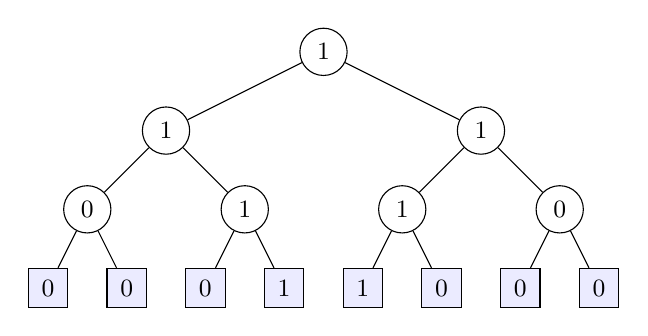
\begin{tikzpicture}[scale=1, every node/.style={font=\small}]
  \node[draw,circle,minimum size=6mm] (r) at (4,3) {1};
  \node[draw,circle,minimum size=6mm] (a) at (2,2) {1};
  \node[draw,circle,minimum size=6mm] (b) at (6,2) {1};
  \node[draw,circle,minimum size=6mm] (a0) at (1,1) {0};
  \node[draw,circle,minimum size=6mm] (a1) at (3,1) {1};
  \node[draw,circle,minimum size=6mm] (b0) at (5,1) {1};
  \node[draw,circle,minimum size=6mm] (b1) at (7,1) {0};
  \foreach \x/\v in {0/0,1/0,2/0,3/1,4/1,5/0,6/0,7/0} {
    \node[draw,rectangle,minimum size=5mm,fill=blue!8] (l\x) at ({0.5+\x},0) {\v};
  }
  \draw (r)--(a); \draw (r)--(b);
  \draw (a)--(a0); \draw (a)--(a1); \draw (b)--(b0); \draw (b)--(b1);
  \draw (a0)--(l0); \draw (a0)--(l1);
  \draw (a1)--(l2); \draw (a1)--(l3);
  \draw (b0)--(l4); \draw (b0)--(l5);
  \draw (b1)--(l6); \draw (b1)--(l7);
\end{tikzpicture}
\caption{A summary tree over $u=8$ for the set $S=\{3,4\}$. Leaves are the bit
vector; each internal node is the OR of its children. Successor of $x=3$:
climb until you find a node whose right subtree is nonempty, cross over, descend
to the leftmost $1$.}
\label{ch21:summary-tree}
\end{figure}

How does this help successor? To find the successor of $x$, start at leaf $x$ and
\emph{climb}. At each step, look at whether the sibling subtree to your right
contains a $1$ (its summary node is $1$). The moment it does, cross into it and
\emph{descend}, always taking the leftmost child that is a $1$, until you reach a
leaf. That leaf is the successor. Climbing is $\Oh(\log u)$ and descending is
$\Oh(\log u)$, so successor is now $\Oh(\log u)$.

That already matches a balanced BST, and we did it without comparisons. But
$\Oh(\log u)$ is not our target; we want $\Oh(\lg\lg u)$. The summary tree has
$\log u$ levels and we walk all of them. To go faster we need a tree that is
\emph{much shallower} -- and the way to get a shallow tree is to give
each node many children instead of two.

\begin{walkbox}
Before reading on, consider this question: the binary summary tree has branching
factor $2$ and height $\log_2 u$. If instead each node had $\sqrt{u}$ children,
how tall would the tree be? Work out the height for $u = 2^{16}$ under branching
factor $2$ versus branching factor $\sqrt{u}=2^8$. The gap you find is exactly
the gap between $\log u$ and the answer we are chasing.
\end{walkbox}

\section{Idea two: split the key, build proto-vEB}

To achieve a tree depth of $\lg\lg u$, we change the branching factor:
instead of branching by $2$, we branch by $\sqrt{u}$. Take a key
$x \in \{0,\dots,u-1\}$ represented by $k = \lg u$ bits, and partition its bit
representation into two equal halves. The \emph{high half} -- the more significant
$k/2 = \tfrac{1}{2}\lg u$ bits -- indexes one of $\sqrt{u}$ ``clusters.'' The
\emph{low half} -- the lower $k/2$ bits -- indexes a position \emph{within} that
cluster, selecting one of $\sqrt{u}$ relative slots.

Formally, with $u = 2^k$ and $\sqrt{u} = 2^{k/2}$, define
\[
  \mathrm{high}(x) = \Big\lfloor \frac{x}{\sqrt{u}} \Big\rfloor,
  \qquad
  \mathrm{low}(x) = x \bmod \sqrt{u},
  \qquad
  \mathrm{index}(h,\ell) = h\sqrt{u} + \ell .
\]
In hardware and modern programming languages, these operations require no arithmetic
division or multiplication. Because $\sqrt{u} = 2^{k/2}$, they correspond to direct
bit-level operations:
\[
  \mathrm{high}(x) = x \gg (k/2), \qquad
  \mathrm{low}(x) = x \ \& \ (2^{k/2} - 1), \qquad
  \mathrm{index}(h, \ell) = (h \ll (k/2)) \mid \ell.
\]
The $\mathrm{index}$ operation reassembles the two halves into the original
integer, so $x = \mathrm{index}(\mathrm{high}(x), \mathrm{low}(x))$ for all $x$.
Each operation executes in $\Oh(1)$ time with single machine instructions.

\begin{example}[Splitting a key]
Let $u = 16$, so $\sqrt{u} = 4$ and keys are $4$-bit numbers. Take $x = 13$,
which in binary is $1101_2$. The high two bits are $11_2 = 3$ and the low two bits
are $01_2 = 1$. Indeed
\[
  \mathrm{high}(13) = \lfloor 13/4 \rfloor = 3, \quad
  \mathrm{low}(13) = 13 \bmod 4 = 1, \quad
  \mathrm{index}(3,1) = 3\cdot 4 + 1 = 13. \checkmark
\]
Key $13$ resides in cluster $3$ at internal offset $1$.
\end{example}

\begin{intuitionbox}
Think of the $u$ keys as the cells of a $\sqrt{u} \times \sqrt{u}$ grid, read
row by row (Figure~\ref{ch21:grid}). The high half of a key is its \emph{row}
(which cluster); the low
half is its \emph{column} (where in the cluster). Key $13$ in a $4\times 4$ grid
sits in row $3$, column $1$. Successor now has a two-part flavor: either the
next key is later in the \emph{same row}, or it is the first key of some
\emph{later nonempty row}.
\end{intuitionbox}

\begin{figure}[h]
\centering
\begin{tikzpicture}[scale=0.85, every node/.style={font=\footnotesize}]
  % column labels (low)
  \foreach \c in {0,1,2,3}{ \node at ({\c+0.5},4.4) {$\ell{=}\c$}; }
  % row labels (high)
  \foreach \r in {0,1,2,3}{ \node at (-0.9,{3.5-\r+0.0}) {$h{=}\r$}; }
  % grid cells: value = h*4 + l, rows top=h0 .. bottom=h3
  \foreach \r in {0,1,2,3}{
    \foreach \c in {0,1,2,3}{
      \pgfmathtruncatemacro{\val}{\r*4+\c}
      \pgfmathtruncatemacro{\hit}{ifthenelse(\val==13,1,0)}
      \node[draw,minimum size=8mm,
            fill={\ifnum\hit=1 quotientorange!35\else blue!4\fi}]
            at ({\c+0.5},{3.5-\r}) {\val};
    }
  }
  \draw[->,thick,structurepurple] (4.6,0.5) -- (4.2,0.5)
        node[right=6pt,structurepurple]{cluster (row) $h$};
  \draw[->,thick,targetgreen] (1.5,-0.4) -- (1.5,0.05)
        node[below=6pt,targetgreen]{offset (column) $\ell$};
\end{tikzpicture}
\caption{The $u=16$ universe drawn as a $\sqrt{u}\times\sqrt{u}=4\times4$ grid,
read row by row. A key's value is $\mathrm{high}\cdot\sqrt u+\mathrm{low}$. Key
$13$ (highlighted) sits in row $h=3$, column $\ell=1$. Clusters are rows;
``successor'' means ``next filled cell scanning left-to-right, top-to-bottom.''}
\label{ch21:grid}
\end{figure}

We now build a recursive structure to match. A \emph{proto-vEB} structure of
size $u$, written $\text{proto-vEB}(u)$, contains:

\begin{itemize}
  \item if $u = 2$ (the base case), a tiny $2$-bit array $A[0..1]$ holding the
        set directly;
  \item otherwise, an array $\mathit{cluster}[0 .. \sqrt{u}-1]$ of
        $\sqrt{u}$ pointers, each to a $\text{proto-vEB}(\sqrt{u})$ holding one
        cluster's worth of keys, plus one extra
        $\text{proto-vEB}(\sqrt{u})$ called $\mathit{summary}$.
\end{itemize}

The $\mathit{summary}$ is the recursive analog of the layered tree's OR-nodes:
$\mathit{summary}$ records \emph{which clusters are nonempty}. Bit
$i$ of the summary is $1$ exactly when $\mathit{cluster}[i]$ contains at
least one key. The summary is itself a proto-vEB over a universe of size
$\sqrt{u}$ -- with one slot per cluster -- so it answers ``which is the next
nonempty cluster?'' by its \emph{own} recursive successor query.
Figure~\ref{ch21:proto-structure} illustrates this two-level recursive structure.

\begin{figure}[h]
\centering
\begin{tikzpicture}[
  scale=0.92,
  every node/.style={font=\footnotesize},
  box/.style={draw=gray!70, rounded corners=2pt, thick},
  sumbox/.style={box, fill=cyan!10},
  clusbox/.style={box, fill=sourceblue!12},
  microbox/.style={box, fill=targetgreen!12},
  lbl/.style={font=\scriptsize\scshape, text=gray!80!black}
]
  % Top Lane: Macro vEB(u)
  \node[lbl, anchor=west] at (-6.2, 3.8) {Macro Structure: $\text{proto-vEB}(u)$};
  \draw[rounded corners=4pt, fill=gray!4, draw=gray!30] (-6.3, 0.95) rectangle (6.3, 3.5);

  \node[box, fill=structurepurple!15, minimum width=2.4cm, minimum height=0.7cm] (root)
    at (0, 2.9) {$\text{proto-vEB}(u)$};

  \node[sumbox, minimum width=2.2cm, minimum height=0.65cm] (sum)
    at (-4.5, 1.8) {$\mathit{summary}$};
  \node[font=\tiny, text=cyan!60!black, below=2pt of sum] {universe $\sqrt{u}$};

  \node[clusbox, minimum width=1.6cm, minimum height=0.65cm] (c0)
    at (-1.8, 1.8) {$\mathit{clus}[0]$};
  \node[clusbox, minimum width=1.6cm, minimum height=0.65cm] (c1)
    at (0.1, 1.8) {$\mathit{clus}[1]$};
  \node at (1.8, 1.8) {$\cdots$};
  \node[clusbox, minimum width=2.2cm, minimum height=0.65cm] (ck)
    at (4.2, 1.8) {$\mathit{clus}[\sqrt{u}-1]$};

  \draw[->, >=stealth, thick, gray!70] (root.south) -| (sum.north);
  \draw[->, >=stealth, thick, gray!70] (root.south) -| (c0.north);
  \draw[->, >=stealth, thick, gray!70] (root.south) -| (c1.north);
  \draw[->, >=stealth, thick, gray!70] (root.south) -| (ck.north);

  % Dashed zoom corridors from clus[1] down to Lane 2
  \draw[dashed, targetgreen!80!black, thick] (c1.south west) -- (-4.5, -0.2);
  \draw[dashed, targetgreen!80!black, thick] (c1.south east) -- (4.5, -0.2);

  % Bottom Lane: Micro recursive expansion of clus[1]
  \node[lbl, anchor=west] at (-6.2, 0.1) {Micro Zoom: Recursive $\text{proto-vEB}(\sqrt{u})$ Substructure};
  \draw[rounded corners=4pt, fill=targetgreen!3, draw=targetgreen!30] (-6.3, -2.68) rectangle (6.3, -0.2);

  \node[box, fill=targetgreen!20, minimum width=2.6cm, minimum height=0.65cm] (subroot)
    at (0, -0.7) {$\mathit{clus}[1]$: size $\sqrt{u}$};

  \node[sumbox, minimum width=2.0cm, minimum height=0.6cm] (subsum)
    at (-3.8, -1.8) {$\mathit{summary}'$};
  \node[font=\tiny, text=cyan!60!black, below=2pt of subsum] {universe $u^{1/4}$};

  \node[microbox, minimum width=1.4cm, minimum height=0.6cm] (sc0)
    at (-1.2, -1.8) {$\mathit{clus}'[0]$};
  \node[microbox, minimum width=1.4cm, minimum height=0.6cm] (sc1)
    at (0.6, -1.8) {$\mathit{clus}'[1]$};
  \node at (2.2, -1.8) {$\cdots$};
  \node[microbox, minimum width=1.8cm, minimum height=0.6cm] (sck)
    at (4.2, -1.8) {$\mathit{clus}'[u^{1/4}-1]$};

  \draw[->, >=stealth, thick, targetgreen!70!black] (subroot.south) -| (subsum.north);
  \draw[->, >=stealth, thick, targetgreen!70!black] (subroot.south) -| (sc0.north);
  \draw[->, >=stealth, thick, targetgreen!70!black] (subroot.south) -| (sc1.north);
  \draw[->, >=stealth, thick, targetgreen!70!black] (subroot.south) -| (sck.north);
\end{tikzpicture}
\caption{The recursive partition of the universe. Top lane: a proto-vEB over universe $u$ contains $\sqrt{u}$ clusters (each of size $\sqrt{u}$) and a summary structure over universe $\sqrt{u}$ recording which clusters are nonempty. Bottom lane: zooming into any cluster shows the same recursive pattern over universe size $u^{1/2}$, branching into $u^{1/4}$ clusters, until the base case $u=2$ is reached.}
\label{ch21:proto-structure}
\end{figure}

\subsection{How tall is this recursion?}

Each level shrinks the universe from $u$ to $\sqrt{u}$. So the universe sizes go
\[
  u,\quad u^{1/2},\quad u^{1/4},\quad u^{1/8},\quad \dots
\]
and we stop when the size reaches $2$. How many square roots does it take to
drive $u$ down to $2$? Write $u = 2^k$. One square root sends $2^k$ to
$2^{k/2}$; that is, it \emph{halves the exponent} $k$. We are done when the
exponent reaches $1$. Halving $k$ down to $1$ takes $\lg k = \lg \lg u$ steps.

\begin{focusbox}
The depth of the recursion is $\lg \lg u$, not $\lg u$. Taking the square root of
the universe at each level halves the \emph{exponent}, and halving repeatedly is a
logarithm. Every $\lg\lg u$ in this chapter comes from this observation, so
check it before continuing.
\end{focusbox}

\begin{example}[Counting the levels]
Let $u = 2^{32}$, so $k = 32$. The universe sizes down the recursion are
\[
  2^{32} \to 2^{16} \to 2^{8} \to 2^{4} \to 2^{2} \to 2^{1}=2.
\]
That is $5$ square-roots, and indeed $\lg\lg u = \lg 32 = 5$. A $32$-bit
universe is only five levels deep. Figure~\ref{ch21:depth} shows this descent
beside the contrast: a binary tree of the same universe is $32$ levels deep.
\end{example}

\begin{figure}[h]
\centering
\begin{tikzpicture}[scale=1, every node/.style={font=\footnotesize}]
  % vEB descent: exponent halves
  \node at (0,3.6) {\textbf{vEB: exponent halves}};
  \foreach \lev/\e in {0/32,1/16,2/8,3/4,4/2,5/1}{
    \node[draw,rounded corners,fill=targetgreen!12,minimum width=1.5cm]
      (v\lev) at (0,{3-0.55*\lev}) {$u=2^{\e}$};
  }
  \foreach \a/\b in {0/1,1/2,2/3,3/4,4/5}{
    \draw[->,targetgreen!70!black] (v\a)--(v\b);
  }
  \node[font=\scriptsize,align=center,targetgreen!60!black]
    at (0,{3-0.55*5-0.5}) {$\lg\lg u=5$ levels};
  % binary tree descent: exponent decrements (shown abbreviated)
  \node at (5,3.6) {\textbf{binary tree: exponent $-1$}};
  \foreach \lev/\e in {0/32,1/31,2/30}{
    \node[draw,rounded corners,fill=trapred!10,minimum width=1.5cm]
      (b\lev) at (5,{3-0.55*\lev}) {$u=2^{\e}$};
  }
  \draw[->,trapred!70!black] (b0)--(b1);
  \draw[->,trapred!70!black] (b1)--(b2);
  \node at (5,{3-0.55*3}) {$\vdots$};
  \node[draw,rounded corners,fill=trapred!10,minimum width=1.5cm]
      (blast) at (5,{3-0.55*4.2}) {$u=2^{1}$};
  \draw[->,trapred!70!black] (b2)--(5,{3-0.55*2.7});
  \draw[->,trapred!70!black] (5,{3-0.55*3.3})--(blast);
  \node[font=\scriptsize,align=center,trapred!70!black]
    at (5,{3-0.55*5-0.0}) {$\lg u=32$ levels};
\end{tikzpicture}
\caption{Why the recursion is shallow. Square-rooting the universe (left)
\emph{halves the exponent} each level, reaching the base in $\lg\lg u$ steps. A
binary tree (right) only \emph{decrements} the exponent, taking $\lg u$ steps.
For $u=2^{32}$ that is $5$ levels versus $32$.}
\label{ch21:depth}
\end{figure}

\section{Proto-vEB operations, and why they are not yet fast enough}

Let us write the operations on proto-vEB and watch carefully where the time
goes. We will find that \textsc{Member} already achieves $\Oh(\lg\lg u)$, whereas
\textsc{Successor} and \textsc{Minimum} still degrade to $\Th(\lg u)$. Seeing
exactly why tells us how to fix the structure.

\subsection{Member}

\begin{algorithm}[H]
\caption{\textsc{proto-vEB-Member}($V, x$)}
\KwIn{A proto-vEB $V$ of size $u$, key $x$.}
\KwOut{\textsc{true} iff $x \in S$.}
\If{$V.u = 2$}{
  \Return $V.A[x]$ \tcp*{base case: read the bit directly}
}
\Return $\textsc{proto-vEB-Member}(V.\mathit{cluster}[\mathrm{high}(x)],\ \mathrm{low}(x))$\;
\end{algorithm}

To test membership you peel off the high half to pick the cluster and recurse on
the low half. The recursion descends one level each call, so it makes
$\lg\lg u$ calls, each $\Oh(1)$. Let $M(u)$ be the time. Then
\[
  M(u) = M(\sqrt{u}) + \Oh(1).
\]
Substitute $m = \lg u$ (so $\lg\sqrt{u} = m/2$) to get
$M(2^m) = M(2^{m/2}) + \Oh(1)$, i.e.\ a function that halves $m$ each step and
adds a constant -- exactly the merge-sort-style recurrence whose answer is
$\Oh(\lg m) = \Oh(\lg\lg u)$. \textsc{Member} is already at the target.

\subsection{Minimum and Maximum -- the slow ones}

To find the minimum, you find the first nonempty cluster (using the summary),
then recurse to find the minimum within it. Watch the cost.

\begin{algorithm}[H]
\caption{\textsc{proto-vEB-Minimum}($V$)}
\KwIn{A proto-vEB $V$ of size $u$.}
\KwOut{The smallest stored key, or \textsc{nil} if empty.}
\If{$V.u = 2$}{
  \lIf{$V.A[0]=1$}{\Return $0$}
  \lElseIf{$V.A[1]=1$}{\Return $1$}
  \lElse{\Return \textsc{nil}}
}
$c \leftarrow \textsc{proto-vEB-Minimum}(V.\mathit{summary})$
  \tcp*{first nonempty cluster}
\lIf{$c = \textsc{nil}$}{\Return \textsc{nil}}
$o \leftarrow \textsc{proto-vEB-Minimum}(V.\mathit{cluster}[c])$
  \tcp*{min within it}
\Return $\mathrm{index}(c, o)$\;
\end{algorithm}

The problem is that this routine makes \emph{two} recursive calls of size
$\sqrt{u}$ on the path to the answer -- one into the summary, one into a cluster.
The recurrence is
\[
  T(u) = 2\,T(\sqrt{u}) + \Oh(1).
\]
With $m = \lg u$ this is $T(2^m) = 2\,T(2^{m/2}) + \Oh(1)$, and substituting
$S(m) = T(2^m)$ gives $S(m) = 2\,S(m/2) + \Oh(1)$, which by the master theorem
(Chapter~4) solves to $S(m) = \Th(m)$. So $T(u) = \Th(\lg u)$, no better than
logarithmic: two calls per level multiply out to $\lg u$ and cancel the benefit
of the shallow recursion.

\begin{trapbox}
The problem is making \emph{more than one} recursive call per level. With one
call per level you pay (depth)$\times\Oh(1) = \Oh(\lg\lg u)$. With two calls per
level the work \emph{branches}, and a branching recursion of depth $\lg\lg u$
with branching factor $2$ does $\Th(\lg u)$ total work. Every fast operation in
the final structure will obey one rule: \textbf{at most one recursive
call into a $\sqrt{u}$-sized substructure.} The rest of the design exists to
satisfy it.
\end{trapbox}

\subsection{Successor -- the bottleneck diagnosed}

Successor has the same problem: branching recursive calls. Tracing the call
path shows why we need to cache the extreme keys. To find
the successor of $x$:

\begin{enumerate}
  \item Look \emph{within $x$'s own cluster} for something bigger than
        $\mathrm{low}(x)$. If found, splice it back with $\mathrm{high}(x)$ and
        return. (One recursive call.)
  \item Otherwise the answer is in a \emph{later} cluster. Ask the summary for
        the next nonempty cluster after $\mathrm{high}(x)$. (A second recursive
        call.) Then take the \emph{minimum} of that cluster. (A \emph{third}
        recursive call!)
\end{enumerate}

\begin{algorithm}[H]
\caption{\textsc{proto-vEB-Successor}($V, x$)}
\KwIn{A proto-vEB $V$ of size $u$, key $x$.}
\KwOut{Smallest stored key $> x$, or \textsc{nil}.}
\If{$V.u = 2$}{
  \lIf{$x = 0$ \textbf{and} $V.A[1]=1$}{\Return $1$}
  \lElse{\Return \textsc{nil}}
}
$o \leftarrow \textsc{proto-vEB-Successor}(V.\mathit{cluster}[\mathrm{high}(x)],\ \mathrm{low}(x))$\;
\If{$o \ne \textsc{nil}$}{
  \Return $\mathrm{index}(\mathrm{high}(x), o)$ \tcp*{found in same cluster}
}
$c \leftarrow \textsc{proto-vEB-Successor}(V.\mathit{summary},\ \mathrm{high}(x))$\;
\lIf{$c = \textsc{nil}$}{\Return \textsc{nil}}
$o' \leftarrow \textsc{proto-vEB-Minimum}(V.\mathit{cluster}[c])$\;
\Return $\mathrm{index}(c, o')$\;
\end{algorithm}

In the worst case this makes recursive calls into the cluster \emph{and} the
summary \emph{and} a minimum. With $\textsc{Minimum}$ itself costing $\Th(\lg u)$
as we just found, the whole procedure costs $\Th(\lg u)$ or more, which is too
slow.

\begin{complexitybox}
\textbf{proto-vEB.}
\textsc{Member}: $\Oh(\lg\lg u)$ -- already perfect.
\textsc{Minimum}/\textsc{Maximum}: $\Th(\lg u)$ -- too slow (two calls/level).
\textsc{Successor}/\textsc{Predecessor}: $\Th(\lg u)$ -- too slow.
\textsc{Insert}/\textsc{Delete}: $\Th(\lg u)$ for the same reason (they recurse
into a cluster \emph{and} update the summary).
The structure is correct but the speed is no better than a BST. Diagnosis:
multiple recursive calls per level.
\end{complexitybox}

\section{Two fixes: cached extremes and a floating minimum}

Consider where the extra recursive calls came from. \textsc{Minimum} made a
call just to find its answer. \textsc{Successor} made a call to \textsc{Minimum}.
\textsc{Insert} made a call into a cluster \emph{and} a call to update the
summary. If we could make \textsc{Minimum} cost $\Oh(1)$, and stop
\textsc{Insert} from always touching both the cluster and the summary, the
budget of ``one recursive call per level'' would be within reach. Two
modifications do exactly this.

\textbf{Fix 1: store the minimum and maximum explicitly.} Give every vEB node two
extra fields, $V.\mathit{min}$ and $V.\mathit{max}$, caching the smallest and
largest keys in that subtree. Now \textsc{Minimum} and \textsc{Maximum} are
$\Oh(1)$ -- just read the field. No recursion at all.

\textbf{Fix 2: the minimum does not live in any cluster.} This is the subtle
part. We adopt the convention that the element stored in
$V.\mathit{min}$ is \emph{not} also stored down in the clusters. It floats at the
top, held only in the $\mathit{min}$ field. (The maximum \emph{is} kept down in
its cluster as well; only the min is special.)

Why do that? Because it lets \textsc{Insert} into an \emph{empty} vEB
stop instantly, and -- more importantly -- it ensures that whenever
\textsc{Insert} has to recurse into a cluster, that cluster was already nonempty,
so the summary does \emph{not} also need a recursive update. We will see in a
moment how this convention reduces two recursive calls to one. The same
applies to \textsc{Successor}: pulling the min out lets it answer most queries by
reading $\mathit{min}$ and $\mathit{max}$ fields without a second descent.

\begin{intuitionbox}
The $\mathit{min}$ field is a doorman standing at the entrance of each vEB node.
Inserting into an empty node? The doorman just remembers you, no need to disturb
anyone inside (the clusters stay untouched, the summary stays untouched).
Inserting a second element? The doorman is already busy, so \emph{now} you go
inside -- but because the node is no longer empty, the summary already knows this
cluster is occupied, so you only ever need to recurse \emph{one} level deeper,
never two. This is what guarantees one recursive call per level.
\end{intuitionbox}

\begin{formalbox}
\textbf{The real vEB tree.} A $\text{vEB}(u)$ structure stores a set
$S \subseteq \{0,\dots,u-1\}$. It has fields $\mathit{min}$, $\mathit{max}$
(each a key or \textsc{nil}). If $u > 2$ it also has
$\mathit{cluster}[0..\sqrt{u}-1]$, each a $\text{vEB}(\sqrt{u})$, and a
$\mathit{summary}$, also a $\text{vEB}(\sqrt{u})$. Invariants:
\begin{itemize}
  \item $\mathit{min}$ holds the smallest key of $S$ and is \emph{not} stored in
        any cluster.
  \item $\mathit{max}$ holds the largest key of $S$ (and, unless it equals
        $\mathit{min}$, \emph{is} also stored in its cluster).
  \item $\mathit{cluster}[i]$ stores exactly $\{\mathrm{low}(x) : x \in S,
        \mathrm{high}(x)=i, x \ne \mathit{min}\}$.
  \item $\mathit{summary}$ stores exactly $\{i : \mathit{cluster}[i]$ is
        nonempty$\}$.
  \item An empty $S$ has $\mathit{min}=\mathit{max}=\textsc{nil}$. A singleton
        $S=\{x\}$ has $\mathit{min}=\mathit{max}=x$ and \emph{all clusters
        empty}.
\end{itemize}
When $u=2$ there are no clusters or summary; the set is fully described by
$\mathit{min}$ and $\mathit{max}$ over $\{0,1\}$.
\end{formalbox}

\section{The fast operations}

Now we rewrite the operations to exploit the two fixes. The recurring pattern to
watch for: \emph{do as much as possible with $\mathit{min}$ and $\mathit{max}$
in $\Oh(1)$, and make at most one genuine recursive call.}

\subsection{Minimum, Maximum, Member}

\textsc{Minimum} and \textsc{Maximum} simply return $V.\mathit{min}$ and
$V.\mathit{max}$: $\Oh(1)$, done. \textsc{Member} is almost as before, but must
first check whether $x$ is the floating minimum or maximum (since those are not
in the clusters):

\begin{algorithm}[H]
\caption{\textsc{vEB-Member}($V, x$)}
\If{$x = V.\mathit{min}$ \textbf{or} $x = V.\mathit{max}$}{\Return \textsc{true}}
\lElseIf{$V.u = 2$}{\Return \textsc{false}}
\lElse{\Return $\textsc{vEB-Member}(V.\mathit{cluster}[\mathrm{high}(x)],\ \mathrm{low}(x))$}
\end{algorithm}

One recursive call per level $\Rightarrow \Oh(\lg\lg u)$, as before.

\subsection{Successor: the centerpiece}

\begin{algorithm}[H]
\caption{\textsc{vEB-Successor}($V, x$)}
\KwIn{vEB $V$ of size $u$, key $x$ (need not be in $S$).}
\KwOut{Smallest key in $S$ that is $> x$, or \textsc{nil}.}
\If{$V.u = 2$}{
  \lIf{$x = 0$ \textbf{and} $V.\mathit{max}=1$}{\Return $1$}
  \lElse{\Return \textsc{nil}}
}
\If{$V.\mathit{min} \ne \textsc{nil}$ \textbf{and} $x < V.\mathit{min}$}{
  \Return $V.\mathit{min}$ \tcp*{the floating min is the answer}
}
$\mathit{maxlow} \leftarrow \textsc{vEB-Maximum}(V.\mathit{cluster}[\mathrm{high}(x)])$\;
\If{$\mathit{maxlow} \ne \textsc{nil}$ \textbf{and} $\mathrm{low}(x) < \mathit{maxlow}$}{
  $o \leftarrow \textsc{vEB-Successor}(V.\mathit{cluster}[\mathrm{high}(x)],\ \mathrm{low}(x))$\;
  \Return $\mathrm{index}(\mathrm{high}(x), o)$ \tcp*{successor is in same cluster}
}
\Else{
  $c \leftarrow \textsc{vEB-Successor}(V.\mathit{summary},\ \mathrm{high}(x))$\;
  \lIf{$c = \textsc{nil}$}{\Return \textsc{nil}}
  \Return $\mathrm{index}(c,\ \textsc{vEB-Minimum}(V.\mathit{cluster}[c]))$\;
}
\end{algorithm}

There are three exits, and only one of them recurses:

\begin{enumerate}
  \item \emph{Cheap shortcut.} If $x$ is smaller than the floating minimum, the
        minimum itself is the successor. $\Oh(1)$, no recursion.
  \item \emph{Same cluster.} We peek at the \emph{maximum} of $x$'s own cluster
        in $\Oh(1)$ (it is just a cached field). If $\mathrm{low}(x)$ is below
        that max, the successor lives in this cluster, so we make one recursive
        \textsc{Successor} call into it -- and \emph{stop}.
  \item \emph{Later cluster.} Otherwise we recurse once into the \emph{summary}
        to find the next nonempty cluster $c$, then read that cluster's
        \textsc{Minimum} -- but \textsc{Minimum} is now $\Oh(1)$! So this branch
        also makes exactly \emph{one} recursive call (into the summary).
\end{enumerate}

The $\Oh(1)$ \textsc{Minimum} (Fix 1) is what lets
branch (3) avoid a second recursion. So no matter which exit we take, we recurse
at most once into a $\sqrt{u}$-sized substructure. The recurrence is finally
\[
  T(u) = T(\sqrt{u}) + \Oh(1),
\]
and we already solved this for \textsc{Member}: $T(u) = \Oh(\lg\lg u)$.
\textsc{Predecessor} is the mirror image (swap min/max, swap successor/maximum)
and is the same cost.

\subsection{A complete numeric trace of Successor}

Let $u = 16$ (so $\sqrt{u}=4$) and $S = \{2, 3, 4, 5, 7, 14, 15\}$. We ask for
$\textsc{Successor}(S, 5)$; the answer should be $7$. Recall the grid view:
$\mathrm{high}(x)=\lfloor x/4\rfloor$ is the row, $\mathrm{low}(x)=x\bmod 4$ is
the column. Figure~\ref{ch21:trace} lays out the structure for this set.

\begin{figure}[h]
\centering
\begin{tikzpicture}[
  scale=0.92,
  every node/.style={font=\footnotesize},
  box/.style={draw=gray!70, rounded corners=2pt, thick},
  valbox/.style={draw=gray!50, rounded corners=2pt, minimum width=1.4cm, minimum height=0.6cm, font=\small},
  lbl/.style={font=\scriptsize\scshape, text=gray!80!black}
]
  % Lane 1: Root metadata
  \node[lbl, anchor=west] at (-6.2, 3.7) {vEB$(16)$ Header Fields};
  \draw[rounded corners=3pt, fill=gray!3, draw=gray!25] (-6.3, 2.6) rectangle (6.3, 3.5);
  \node[box, fill=structurepurple!15, minimum width=4.0cm, minimum height=0.65cm] (min)
    at (-2.5, 3.05) {$\mathit{min} = 2$ \scriptsize(floating; not in clus)};
  \node[box, fill=quotientorange!15, minimum width=3.2cm, minimum height=0.65cm] (max)
    at (2.5, 3.05) {$\mathit{max} = 15$};

  % Lane 2: Summary
  \node[lbl, anchor=west] at (-6.2, 2.1) {Summary Structure (Universe $\sqrt{u}=4$: tracks which clusters are nonempty)};
  \draw[rounded corners=3pt, fill=cyan!3, draw=cyan!25] (-6.3, 0.95) rectangle (6.3, 1.95);

  % Summary slots aligned directly above clusters
  \node[valbox, fill=cyan!25, text=cyan!90!black, draw=cyan!70] (s0) at (-4.5, 1.45) {$\mathit{summary}[0] = 1$};
  \node[valbox, fill=cyan!25, text=cyan!90!black, draw=cyan!70] (s1) at (-1.5, 1.45) {$\mathit{summary}[1] = 1$};
  \node[valbox, fill=gray!12, text=gray!50, draw=gray!40] (s2) at (1.5, 1.45) {$\mathit{summary}[2] = 0$};
  \node[valbox, fill=cyan!25, text=cyan!90!black, draw=cyan!70] (s3) at (4.5, 1.45) {$\mathit{summary}[3] = 1$};

  % Lane 3: Cluster Array
  \node[lbl, anchor=west] at (-6.2, 0.45) {Cluster Array ($\sqrt{u}=4$ Clusters of Universe $4$)};
  \draw[rounded corners=3pt, fill=sourceblue!3, draw=sourceblue!25] (-6.3, -1.8) rectangle (6.3, 0.3);

  % Cluster 0
  \node[box, fill=sourceblue!10, minimum width=2.7cm, minimum height=1.65cm] (c0box) at (-4.5, -0.75) {};
  \node[font=\scriptsize\bfseries, text=sourceblue!80!black, align=center] at (-4.5, -0.15) {clus[0]\\[-2pt]\tiny keys $\in [0..3]$};
  \node[font=\tiny] at (-4.5, -0.58) {$\mathit{min}{=}\mathit{max}{=}3$};
  \node[font=\tiny, text=gray!75!black] at (-4.5, -0.92) {lows stored: $\{3\}$};
  \node[font=\tiny, text=structurepurple!80!black] at (-4.5, -1.25) {(key $2$ is root min)};

  % Cluster 1
  \node[box, fill=sourceblue!10, minimum width=2.7cm, minimum height=1.65cm] (c1box) at (-1.5, -0.75) {};
  \node[font=\scriptsize\bfseries, text=sourceblue!80!black, align=center] at (-1.5, -0.15) {clus[1]\\[-2pt]\tiny keys $\in [4..7]$};
  \node[font=\tiny] at (-1.5, -0.58) {$\mathit{min}{=}0$, $\mathit{max}{=}3$};
  \node[font=\tiny, text=gray!75!black] at (-1.5, -0.92) {lows stored: $\{0, 1, 3\}$};
  \node[font=\tiny, text=gray!70!black] at (-1.5, -1.25) {keys $4, 5, 7$};

  % Cluster 2
  \node[box, fill=gray!8, draw=gray!40, minimum width=2.7cm, minimum height=1.65cm] (c2box) at (1.5, -0.75) {};
  \node[font=\scriptsize\bfseries, text=gray!60!black, align=center] at (1.5, -0.15) {clus[2]\\[-2pt]\tiny keys $\in [8..11]$};
  \node[font=\tiny, text=gray!55] at (1.5, -0.65) {$\mathit{min}{=}\textsc{nil}$};
  \node[font=\tiny, text=gray!55] at (1.5, -1.05) {$\emptyset$ (empty)};

  % Cluster 3
  \node[box, fill=sourceblue!10, minimum width=2.7cm, minimum height=1.65cm] (c3box) at (4.5, -0.75) {};
  \node[font=\scriptsize\bfseries, text=sourceblue!80!black, align=center] at (4.5, -0.15) {clus[3]\\[-2pt]\tiny keys $\in [12..15]$};
  \node[font=\tiny] at (4.5, -0.58) {$\mathit{min}{=}2$, $\mathit{max}{=}3$};
  \node[font=\tiny, text=gray!75!black] at (4.5, -0.92) {lows stored: $\{2, 3\}$};
  \node[font=\tiny, text=gray!70!black] at (4.5, -1.25) {keys $14, 15$};

  % Dedicated vertical arrows connecting summary slots to clusters
  \draw[->, >=stealth, thick, cyan!80!black] (s0.south) -- (c0box.north);
  \draw[->, >=stealth, thick, cyan!80!black] (s1.south) -- (c1box.north);
  \draw[->, >=stealth, thick, cyan!80!black] (s3.south) -- (c3box.north);
\end{tikzpicture}
\caption{The vEB$(16)$ for $S=\{2,3,4,5,7,14,15\}$ displayed with dedicated horizontal lanes. The overall minimum key, $2$, floats in $\mathit{min}$ and is \emph{not} stored in any cluster. Keys $\{3,4,5,7,14,15\}$ map to clusters by their high half, where they are stored as low offsets. The summary structure tracks nonempty clusters $0, 1, 3$. Cluster $2$ contains no keys.}
\label{ch21:trace}
\end{figure}

\begin{labbox}
\textbf{Trace.} The top vEB has $\mathit{min}=2$ (floating, not in any cluster).
The remaining keys $\{3,4,5,7,14,15\}$ distribute into clusters by their high
half:
\[
\begin{array}{l|l|l}
\text{cluster } i & \text{keys with high}=i & \text{stored lows} \\\hline
0 & 3 & \{3\}\ (\text{since } \mathrm{low}(3)=3)\\
1 & 4,5,7 & \{0,1,3\}\\
3 & 14,15 & \{2,3\}\\
\end{array}
\]
Cluster $2$ is empty. The summary stores $\{0,1,3\}$ (the nonempty clusters),
with its own floating $\mathit{min}=0$.

Now run $\textsc{vEB-Successor}(V, 5)$:
\begin{enumerate}
  \item $u=16 \ne 2$. Is $5 < V.\mathit{min}=2$? No.
  \item $\mathrm{high}(5)=1$, $\mathrm{low}(5)=1$. Peek at
        $\textsc{Maximum}(\mathit{cluster}[1])$. Cluster $1$ holds lows
        $\{0,1,3\}$ so its max is $3$. Is $\mathrm{low}(5)=1 < 3$? Yes ---
        the successor is in the same cluster.
  \item Recurse: $\textsc{vEB-Successor}(\mathit{cluster}[1],\ 1)$. Inside,
        the next low after $1$ among $\{0,1,3\}$ is $3$. Return $3$.
  \item Splice back: $\mathrm{index}(\mathrm{high}=1, o=3) = 1\cdot 4 + 3 = 7$.
\end{enumerate}
Answer: $7$. \checkmark\ Exactly one recursive descent was made.

\textbf{Second trace}, crossing clusters: $\textsc{vEB-Successor}(V, 7)$, answer
should be $14$.
\begin{enumerate}
  \item $7 < 2$? No. $\mathrm{high}(7)=1$, $\mathrm{low}(7)=3$.
  \item $\textsc{Maximum}(\mathit{cluster}[1]) = 3$. Is $\mathrm{low}(7)=3 < 3$?
        No. So look in a \emph{later} cluster.
  \item Recurse into summary: $\textsc{vEB-Successor}(\mathit{summary}, 1)$.
        Summary holds $\{0,1,3\}$; the next after $1$ is $3$. So $c=3$.
  \item $\textsc{Minimum}(\mathit{cluster}[3])$: cluster $3$ holds lows
        $\{2,3\}$, min is $2$ ($\Oh(1)$ field read). Splice:
        $\mathrm{index}(3, 2) = 3\cdot 4 + 2 = 14$.
\end{enumerate}
Answer: $14$. \checkmark
\end{labbox}

\subsection{Insert: one recursion via the doorman}

\begin{algorithm}[H]
\caption{\textsc{vEB-Insert}($V, x$)}
\If{$V.\mathit{min} = \textsc{nil}$}{
  $V.\mathit{min} \leftarrow V.\mathit{max} \leftarrow x$
  \tcp*{empty: just seat the doorman, $\Oh(1)$, stop}
  \Return
}
\If{$x < V.\mathit{min}$}{
  swap $x \leftrightarrow V.\mathit{min}$
  \tcp*{new smallest: displace the old min downward}
}
\If{$V.u > 2$}{
  \eIf{$\textsc{vEB-Minimum}(V.\mathit{cluster}[\mathrm{high}(x)]) = \textsc{nil}$}{
    $\textsc{vEB-Insert}(V.\mathit{summary},\ \mathrm{high}(x))$
      \tcp*{cluster was empty: update summary}
    set $\mathit{cluster}[\mathrm{high}(x)].\mathit{min} =
        \mathit{cluster}[\mathrm{high}(x)].\mathit{max} = \mathrm{low}(x)$\;
  }{
    $\textsc{vEB-Insert}(V.\mathit{cluster}[\mathrm{high}(x)],\ \mathrm{low}(x))$
      \tcp*{cluster nonempty: recurse into it}
  }
}
\lIf{$x > V.\mathit{max}$}{$V.\mathit{max} \leftarrow x$}
\end{algorithm}

This mutual exclusion between the summary update and the cluster descent is what
makes the floating minimum convention work. The two recursive
calls -- one into the summary, one into the cluster -- live in \emph{opposite}
branches of an \texttt{if/else}. They never both fire on the same level:

\begin{itemize}
  \item If the target cluster is \emph{empty}, we recurse into the summary to
        record that it just became nonempty, and we seat the cluster's doorman
        in $\Oh(1)$ \emph{without} recursing into the cluster. Inserting into an
        empty vEB is $\Oh(1)$ (the first \texttt{if}), so the summary call's own
        deeper recursion also terminates immediately at its next level.
  \item If the target cluster is \emph{nonempty}, the summary already knows about
        it, so we skip the summary entirely and recurse only into the cluster.
\end{itemize}

Figure~\ref{ch21:fig-insert-cases} contrasts the two execution paths: in both branches, exactly one operation recurses, while the other is either omitted or finishes in $\Oh(1)$ time.

\begin{figure}[htbp]
\centering
\begin{tikzpicture}[
  scale=0.92,
  every node/.style={font=\footnotesize},
  box/.style={draw=gray!60, rounded corners=3pt, thick},
  action/.style={draw=gray!50, rounded corners=2pt, minimum width=5.6cm, minimum height=0.9cm, align=center},
  hdr/.style={font=\small\bfseries, text=gray!80!black}
]
  % Case 1 Box
  \draw[box, fill=sourceblue!3, draw=sourceblue!40] (-6.75, -2.4) rectangle (-0.25, 2.4);
  \node[hdr, text=sourceblue!90!black] at (-3.5, 2.0) {Case A: Target \texttt{clus[h]} is Empty};
  \node[font=\scriptsize, text=gray!70!black] at (-3.4, 1.45) {($\textsc{vEB-Minimum}(\texttt{clus}[h]) = \textsc{nil}$)};

  \node[action, fill=structurepurple!15, draw=structurepurple!60] at (-3.4, 0.45) {
    \textbf{1. Summary update} (recursive)\\[-1pt]
    $\textsc{vEB-Insert}(V.\mathit{summary},\ h)$ \quad {\scriptsize\color{structurepurple!80!black}[$T(\sqrt{u})$]}
  };

  \node[action, fill=targetgreen!15, draw=targetgreen!60] at (-3.4, -0.75) {
    \textbf{2. Cluster write} (base case)\\[-1pt]
    $\texttt{clus}[h].\mathit{min} \leftarrow \texttt{clus}[h].\mathit{max} \leftarrow \ell$ \quad {\scriptsize\color{targetgreen!80!black}[$\Oh(1)$]}
  };

  \node[draw=sourceblue!60, fill=sourceblue!15, rounded corners=2pt, font=\scriptsize\bfseries, text=sourceblue!90!black]
    at (-3.4, -1.85) {Active recursive calls: 1};

  % Case 2 Box
  \draw[box, fill=quotientorange!3, draw=quotientorange!40] (0.25, -2.4) rectangle (6.75, 2.4);
  \node[hdr, text=quotientorange!90!black] at (3.5, 2.0) {Case B: Target \texttt{clus[h]} is Nonempty};
  \node[font=\scriptsize, text=gray!70!black] at (3.4, 1.45) {($\textsc{vEB-Minimum}(\texttt{clus}[h]) \neq \textsc{nil}$)};

  \node[action, fill=gray!8, draw=gray!30, text=gray!50] at (3.4, 0.45) {
    \textbf{1. Summary update} (skipped)\\[-1pt]
    Cluster $h$ already active \quad {\scriptsize[$\Oh(0)$]}
  };

  \node[action, fill=structurepurple!15, draw=structurepurple!60] at (3.4, -0.75) {
    \textbf{2. Cluster descent} (recursive)\\[-1pt]
    $\textsc{vEB-Insert}(\texttt{clus}[h],\ \ell)$ \quad {\scriptsize\color{structurepurple!80!black}[$T(\sqrt{u})$]}
  };

  \node[draw=quotientorange!60, fill=quotientorange!15, rounded corners=2pt, font=\scriptsize\bfseries, text=quotientorange!90!black]
    at (3.4, -1.85) {Active recursive calls: 1};

  % Bottom banner
  \node[draw=gray!40, fill=gray!5, rounded corners=3pt, font=\footnotesize, align=center, minimum width=12.8cm, minimum height=0.65cm]
    at (0, -3.05) {
      \textbf{Key Invariant:} Exactly one branch recurses $\implies T(u) = T(\sqrt{u}) + \Oh(1) = \Oh(\lg\lg u)$
    };
\end{tikzpicture}
\caption{The mutual-exclusion invariant in \textsc{vEB-Insert}. When cluster $h$ is empty (left), the recursive call goes to the summary while the cluster itself is initialized in $\Oh(1)$ as a doorman base case. When cluster $h$ is nonempty (right), the summary requires no update, and the single recursive call descends into cluster $h$. In both cases, exactly one non-$\Oh(1)$ recursive call is issued per level.}
\label{ch21:fig-insert-cases}
\end{figure}

So along the actual chain of nested calls, only one ``real'' (non-$\Oh(1)$)
recursive call happens per level. The recurrence is again
$T(u) = T(\sqrt{u}) + \Oh(1) = \Oh(\lg\lg u)$.

\begin{trapbox}
A tempting misreading: ``\textsc{Insert} makes two recursive calls, so it must be
$\Th(\lg u)$ like proto-vEB.'' In fact the two calls are in mutually exclusive
branches, and the branch that recurses into the summary does so only when the
cluster is empty -- which makes the \emph{paired} cluster operation $\Oh(1)$. The
``$\le$ one expensive recursive call per level'' invariant holds. Always check
\emph{which} calls can fire \emph{together on a path}, not how many appear in the
source.
\end{trapbox}

\subsection{Delete: the bookkeeping is heavier but the bound holds}

\textsc{Delete} is the fiddliest operation because removing the floating minimum
forces us to promote a new one from the clusters. The structure of the
argument is identical, though: only one nontrivial recursive call fires per
level.

\begin{algorithm}[H]
\caption{\textsc{vEB-Delete}($V, x$)}
\If{$V.\mathit{min} = V.\mathit{max}$}{
  $V.\mathit{min} \leftarrow V.\mathit{max} \leftarrow \textsc{nil}$
  \tcp*{only one element; now empty}
  \Return
}
\If{$V.u = 2$}{
  \lIf{$x=0$}{$V.\mathit{min}\leftarrow 1$}\lElse{$V.\mathit{min}\leftarrow 0$}
  $V.\mathit{max}\leftarrow V.\mathit{min}$\; \Return
}
\If{$x = V.\mathit{min}$}{
  $c \leftarrow \textsc{vEB-Minimum}(V.\mathit{summary})$
    \tcp*{first nonempty cluster}
  $x \leftarrow \mathrm{index}(c,\ \textsc{vEB-Minimum}(V.\mathit{cluster}[c]))$\;
  $V.\mathit{min} \leftarrow x$
    \tcp*{promote: this key will be removed from its cluster below}
}
$\textsc{vEB-Delete}(V.\mathit{cluster}[\mathrm{high}(x)],\ \mathrm{low}(x))$\;
\If{$\textsc{vEB-Minimum}(V.\mathit{cluster}[\mathrm{high}(x)]) = \textsc{nil}$}{
  $\textsc{vEB-Delete}(V.\mathit{summary},\ \mathrm{high}(x))$
    \tcp*{cluster emptied: clear its summary bit}
  \If{$x = V.\mathit{max}$}{
    \emph{recompute }$V.\mathit{max}$\emph{ from summary/clusters (}$\Oh(1)$\emph{ field reads)}\;
  }
}
\lElseIf{$x = V.\mathit{max}$}{
  $V.\mathit{max} \leftarrow \mathrm{index}(\mathrm{high}(x),\ \textsc{vEB-Maximum}(V.\mathit{cluster}[\mathrm{high}(x)]))$
}
\end{algorithm}

There appear to be two recursive \textsc{Delete} calls (cluster, then possibly
summary), so we must argue carefully that they do not both genuinely recurse on
the same path. The second one fires only when the cluster became \emph{empty}
after the first deletion. But deleting the last element of a cluster
(\textsc{Delete} on a one-element vEB) hits the very first \texttt{if} and costs
$\Oh(1)$ -- it does not recurse deeper. So the expensive deletion happens in
\emph{either} the cluster \emph{or} the summary, never both at full depth. Once
more $T(u) = T(\sqrt{u}) + \Oh(1) = \Oh(\lg\lg u)$.

\begin{complexitybox}
\textbf{vEB (final).} Every operation -- \textsc{Member}, \textsc{Insert},
\textsc{Delete}, \textsc{Minimum}, \textsc{Maximum}, \textsc{Successor},
\textsc{Predecessor} -- runs in $\Oh(\lg\lg u)$ worst-case time, governed by the
single recurrence $T(u) = T(\sqrt{u}) + \Oh(1)$. The price is space (next
section) and a fixed integer universe.
\end{complexitybox}

\section{Solving the recurrence, once and for all}

We keep invoking ``$T(u) = T(\sqrt{u}) + \Oh(1) = \Oh(\lg\lg u)$.'' Let us
solve it, because the same substitution handles several other recurrences in
this book.

The difficulty is the $\sqrt{u}$, which is awkward to iterate. A change of
variables turns the square root into a halving. Let
\[
  m = \lg u, \qquad\text{equivalently } u = 2^m.
\]
Then $\sqrt{u} = u^{1/2} = 2^{m/2}$, so its log is $m/2$. Define
$S(m) = T(2^m)$. The recurrence $T(u) = T(\sqrt{u}) + \Oh(1)$ becomes
\[
  S(m) = T(2^m) = T(2^{m/2}) + \Oh(1) = S(m/2) + \Oh(1).
\]
That is a recurrence that \emph{halves $m$} and adds a constant -- precisely the
shape of binary search. By the master theorem (Chapter~4, case 2 with
$a=1, b=2, f=\Oh(1)$), it solves to
\[
  S(m) = \Oh(\lg m).
\]
Unwinding the substitution, $m = \lg u$, so
\[
  T(u) = S(\lg u) = \Oh(\lg \lg u).
\]

\begin{walkbox}
On your walk, prove the $\Oh(\lg m)$ from scratch by unrolling, no master
theorem. Write $S(m) = S(m/2)+c = S(m/4)+2c = S(m/8)+3c = \cdots$. After $t$
steps the argument is $m/2^t$ and the accumulated cost is $tc$. The recursion
stops when $m/2^t$ reaches the base ($1$), i.e.\ when $t = \lg m$. So
$S(m) = \Th(\lg m)\cdot c = \Oh(\lg m)$. This rederives the depth
$\lg\lg u$.
\end{walkbox}

\section{The cost of all this: space}

A $\text{vEB}(u)$ recursively contains $\sqrt{u}$ cluster
substructures plus one summary substructure, each a $\text{vEB}(\sqrt{u})$, and
all of them are \emph{allocated up front} -- even the clusters that hold nothing.
Let $P(u)$ be the space. Then
\[
  P(u) = (\sqrt{u} + 1)\,P(\sqrt{u}) + \Oh(1).
\]
This solves to $P(u) = \Th(u)$. The structure occupies space proportional to the
\emph{entire universe}, whether you store one key or a million.

\begin{trapbox}
$\Th(u)$ space is the catch that limits where vEB is usable. For $u=2^{32}$ that
is billions of cells -- gigabytes -- even to store ten keys. The remedy in
practice is to replace the array of $\sqrt{u}$ cluster pointers with a
\emph{hash table} (Chapter~11) keyed by cluster index, allocating a cluster only
when it first becomes nonempty. That cuts space to $\Oh(n)$ (proportional to the
keys actually present) while keeping the $\Oh(\lg\lg u)$ time
\emph{expected}. CLRS develops this as the related ``$y$-fast trie'' direction in
its problems and chapter notes.
\end{trapbox}

\begin{aestheticbox}
The general lesson: \emph{when your keys
are not abstract, exploit their structure.} The comparison lower bound only binds
when all you can do is ask ``is $a < b$?''. Once you can
\emph{index by a key} -- use the key as an address -- faster algorithms become
possible. This is the same insight behind counting sort and radix sort (Chapter~8) and
behind direct-address tables (Chapter~11). vEB is the most sophisticated member
of that family: it indexes \emph{recursively}, by half the key at a time.
\end{aestheticbox}

\begin{historybox}
Peter van Emde Boas presented the first version of this data structure in 1975 at the IEEE Symposium on Foundations of Computer Science (with full journal versions co-authored with Roman Kaas and Erik Zijlstra appearing in 1977). His goal was to determine whether a priority queue on integers could break the $\Omega(\log n)$ comparison bound on a realistic machine model. By viewing integers as hierarchical coordinate pairs through square-root decomposition ($\sqrt{u}$ clusters of capacity $\sqrt{u}$), caching extremes, and using bitwise shifting to locate clusters in constant time, he showed that all priority-queue and predecessor queries can run in $O(\log \log u)$ time.

The structure had a serious practical limitation: the tree required $\Theta(u)$ words of memory even when storing only a handful of keys, rendering it prohibitive on large universes such as 64-bit address spaces. This motivated decades of research into integer data structures. In 1983, Dan Willard introduced $x$-fast and $y$-fast tries, which combine prefix trees with dynamic hashing to shrink the space requirement to $O(n)$ while preserving $O(\log \log u)$ expected time. In 1993, Michael Fredman and Dan Willard introduced fusion trees, which pack multiple keys into a single machine word to achieve $O(\log n / \log w)$ time per operation on a $w$-bit word RAM, proving that integers can be sorted faster than comparison trees without bounding the universe size. Later cell-probe lower bounds by Mihai P\v{a}tra\c{s}cu and Mikkel Thorup proved that the double-logarithmic query time of van Emde Boas trees is optimal for any data structure occupying space polynomial in $n$. Modern research focuses on cache-oblivious layouts and closing constant-factor instruction penalties on real CPUs. In CLRS (3rd edition, Chapter~20), the structure is developed through the same progression: bit vector to binary summary tree, proto-vEB, and finally the full recursive vEB with cached extremes.
\end{historybox}

\section{Recap: the chain of ideas}

Each step below fixes the flaw in the step before it.

\begin{focusbox}
\begin{enumerate}
  \item \textbf{Bit vector} ($\Oh(u)$ successor): $\Oh(1)$ membership but
        successor scans a flat array.
  \item \textbf{Binary summary tree} ($\Oh(\lg u)$): add OR-summaries to get
        shortcuts, but the tree is $\lg u$ tall.
  \item \textbf{Square-root split / proto-vEB} (depth $\lg\lg u$): branch by
        $\sqrt{u}$ so the recursion is only $\lg\lg u$ deep -- but operations
        make $\ge 2$ recursive calls per level, so they still cost $\Th(\lg u)$.
  \item \textbf{Stored $\mathit{min}/\mathit{max}$ + floating min} ($\Oh(\lg\lg
        u)$): cache min/max for $\Oh(1)$ access, and keep the min out of the
        clusters, so every operation makes \emph{exactly one} recursive call per
        level. Recurrence $T(u)=T(\sqrt u)+\Oh(1)=\Oh(\lg\lg u)$.
\end{enumerate}
The rule behind every step: \emph{one recursive call into a
$\sqrt{u}$-substructure per level.} The rest is bookkeeping that maintains that
rule.
\end{focusbox}

This chapter ends our study of advanced data structures. In Part~6, we turn to graphs and network algorithms, beginning in Chapter~22 with representations of graphs and the two basic ways to traverse them---breadth-first and depth-first search.

\section{Exercises}

\begin{exercise}[Counting the levels]
For each universe size $u \in \{4,\ 16,\ 256,\ 2^{16},\ 2^{64}\}$, write out the
sequence of universe sizes down the vEB recursion ($u \to \sqrt u \to \cdots \to
2$) and confirm the number of levels equals $\lg\lg u$. Which of these would have
operations costing more than $6$ ``levels'' of work? (Warmup.)
\end{exercise}

\begin{exercise}[Splitting keys]
Let $u = 256$, so $\sqrt u = 16$. Compute $\mathrm{high}(x)$, $\mathrm{low}(x)$,
and verify $\mathrm{index}(\mathrm{high}(x),\mathrm{low}(x)) = x$ for
$x \in \{0, 17, 200, 255\}$. Describe $\mathrm{high}$ and $\mathrm{low}$ purely
as bit operations (shift / mask) on the $8$-bit value $x$. (Warmup.)
\end{exercise}

\begin{exercise}[Why two calls per level is fatal]
Solve each recurrence by the $m=\lg u$ substitution and state the closed form:
(a) $T(u)=T(\sqrt u)+\Oh(1)$; (b) $T(u)=2\,T(\sqrt u)+\Oh(1)$;
(c) $T(u)=\sqrt u\,T(\sqrt u)+\Oh(1)$. Match each to one of the structures in the
chapter (final vEB, proto-vEB minimum, total space). (Medium.)
\end{exercise}

\begin{exercise}[Trace Successor]
Let $u=16$ and $S=\{1,2,6,9,13\}$. Lay out the clusters and the summary
(recall that the floating minimum is not stored in any cluster). Trace
\textsc{vEB-Successor}$(V, x)$ for $x = 2$, $x = 6$, and $x = 9$, naming which of
the three exits fires each time and how many recursive descents occur.
(Medium.)
\end{exercise}

\begin{exercise}[Trace Insert]
Starting from an empty $\text{vEB}(16)$, insert the keys $5, 2, 8, 5, 0$ in that
order (the second $5$ is a no-op; explain why). After each insertion, write down
$\mathit{min}$, $\mathit{max}$, the contents of each cluster, and the summary.
Point out every insertion that took $\Oh(1)$ time because it hit the empty-node
fast path. (Medium.)
\end{exercise}

\begin{exercise}[The floating minimum, examined]
Explain in your own words why \textsc{vEB-Insert} into an \emph{empty} node is
$\Oh(1)$, and why this single fact is what keeps \textsc{Insert}'s recurrence at
$T(u)=T(\sqrt u)+\Oh(1)$ rather than $T(u)=2\,T(\sqrt u)+\Oh(1)$. What would
break if we instead stored the minimum down in its cluster like every other
element? (Medium.)
\end{exercise}

\begin{exercise}[Predecessor by mirror]
\textsc{vEB-Predecessor} is the mirror of \textsc{Successor}, but there is one
asymmetry: it has a special case that \textsc{Successor} does not, involving
$\mathit{min}$. Write \textsc{vEB-Predecessor} in full pseudocode and explain the
extra case. Hint: the floating $\mathit{min}$ is below everything in the
clusters, so when the cluster search fails, you must still check whether $x$ is
greater than $\mathit{min}$. (Medium-hard.)
\end{exercise}

\begin{exercise}[Trace Delete, including a promotion]
Take $u=16$ and $S=\{0,3,4,11\}$ with the structure correctly built. Trace
$\textsc{vEB-Delete}(V, 0)$. Since $0$ is the floating minimum, follow the
promotion: which key becomes the new $\mathit{min}$, and from which cluster is it
then removed? Show the clusters and summary before and after. (Hard.)
\end{exercise}

\begin{exercise}[Space recurrence]
Set up and solve the space recurrence $P(u) = (\sqrt u + 1)P(\sqrt u)+\Oh(1)$ to
show $P(u)=\Th(u)$. Then estimate the space, in cells, for $u = 2^{20}$ holding a
set of just $3$ keys, and contrast with a balanced BST holding the same $3$ keys.
What does this tell you about when to reach for a vEB tree? (Hard.)
\end{exercise}

\begin{exercise}[From $\Th(u)$ space to $\Oh(n)$ space]
Sketch how replacing the array $\mathit{cluster}[0..\sqrt u - 1]$ with a hash
table (Chapter~11), allocating a cluster only on its first nonempty insert,
reduces space to $\Oh(n)$. Which time bounds become \emph{expected} rather than
worst-case, and why? (Challenge.)
\end{exercise}

\begin{exercise}[Successor without stored max]
Suppose you kept the floating $\mathit{min}$ trick but did \emph{not} cache
$\mathit{max}$ -- you would have to compute a cluster's maximum by a recursive
call. Show that \textsc{Successor} then makes two genuine recursive calls in its
``same cluster'' branch (the max query plus the successor query), and that its
running time degrades to $\Th(\lg u)$. This isolates exactly why caching
$\mathit{max}$ in addition to $\mathit{min}$ is essential. (Challenge.)
\end{exercise}
